\section{Closed-loop issue with regular \ac{DeePC}}\label{sec:CL_ID_issue}
To demonstrate and compare the performance of \ac{DeePC} and \ac{CL-DeePC} under the influence of feedback, different simulation studies are performed. The simulated plant is a marginally stable 5th-order 

\begin{align}\label{eq:SysFavoreel}
\scriptsize
\begin{array}{lll}
    A = \begin{bmatrix}
        4.40 & 1 & 0 & 0 & 0\\
       -8.09 & 0 & 1 & 0 & 0\\
        7.83 & 0 & 0 & 1 & 0\\
       -4.00 & 0 & 0 & 0 & 1\\
        0.86 & 0 & 0 & 0 & 0
    \end{bmatrix}\!,&
    B = \begin{bmatrix}
        0.00098\\
        0.01299\\
        0.01859\\
        0.0033\\
       -0.00002
    \end{bmatrix}\!,&C = \begin{bmatrix}
        1 \\ 0 \\ 0\\ 0\\ 0
    \end{bmatrix}^\top\mkern-7mu,\\
    K = \begin{bmatrix}
        2.3 & -6.64 & 7.515 & -4.0146 & 0.86336
    \end{bmatrix}^\top\mkern-7mu,\span
    &D=0,
\end{array}
\end{align}

% ------------------------- Figure --------------------------
\begin{figure}
\begin{center}
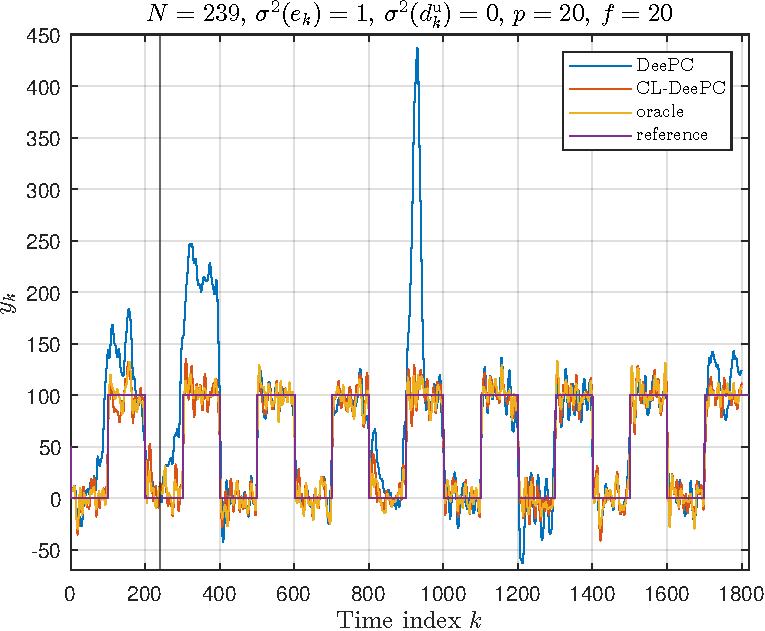
\includegraphics[width=\columnwidth]{results/figures/DeePC_CL_ID_issue_Re_1.mat_Nbar_239_p_20_f_20_Ru_1_Rdu_0_Q_100_R_0_dR_10.pdf}    % The printed column  
\caption{Reference tracking by adaptive \ac{DeePC} and \ac{CL-DeePC} using \ac{IVs} with $p=f=20$, $\bar{N}=539$, $Q=100$, $R=0$, $R^\Delta=10$, $|u_k-u_{k-1}|\leq3.75$, and $|u_k|\leq15$ for the system defined by \eqref{eq:SysFavoreel} with $\text{var}(e_k)=0.5$. %Both controllers are initialized by persistently exciting open-loop data. After $\bar{N}$ samples at the black vertical line, all used input-output data has been collected in closed-loop.
Unlike with \ac{CL-DeePC}, reference tracking by \ac{DeePC} deteriorates because of the closed-loop identification problem.}  % width is 8.4 cm.
\label{fig:CL_Problem_Solution}                                 % Size the figures 
\end{center}                                 % accordingly.
\end{figure}
% -----------------------------------------------------------